\documentclass[a4paper,11pt]{article}

\usepackage{amsmath,amsfonts}
\usepackage{biblatex}
\addbibresource{ref.bib}
\usepackage{booktabs}
\usepackage[font=normalsize]{caption}
\usepackage{float}
\usepackage{graphicx}
\usepackage[utf8]{inputenc}
\usepackage[ignoreunlbld]{refcheck}
\usepackage{longtable}
\setkeys{Gin}{width=.8\textwidth}
\usepackage{nicefrac}
\usepackage{subcaption}

\font\Bbb=msbm10 at 11pt
\def\QQ{\mbox{\Bbb Q}}
\def\RR{\mbox{\Bbb R}}

\graphicspath{ {./images/} }

\DeclareMathOperator{\E}{\mathbb{E}}

\title{Newsvendor Problems: Using Stochastic Programming to Inform Marketing Decisions}

\author{Congzheng Liu\thanks{Department of Management Science,
Lancaster University, Lancaster LA1 4YX, UK.
Email: {\tt \{c.liu19,a.n.letchford,i.svetunkov\}@lancaster.ac.uk}}
\and Adam N.\ Letchford$^*$ \and Ivan Svetunkov$^*$} % end author list

\date{Draft, 26th March 2021}

\begin{document}
\maketitle

\begin{abstract}
Although the literature on newsvendor problems is vast, not much attention has been paid to the question of how to coordinate the marketing and inventory functions in a business when faced with a complex newsvendor problem. We present an approach, based on stochastic programming, that enables one to estimate the changes in expected profit that would arise from specific marketing interventions. The approach is applicable to a wide range of problems, including problems with multiple item types, side constraints, correlated demands, cross-price elasticities and different noise distributions.
\\*[2mm]
{\bf Keywords:} newsvendor problems; stochastic programming; marketing; inventory control 
\end{abstract}

%%%%%%%%%%%%%%%%%%%%%%%%%%%%%%%%%%
\section{Introduction}

Marketing and inventory control are two crucial functions in retailing sectors. It is clear that decisions made by marketing team can have implications for inventory control. For example, high uncertainty in demand can lead to sub-optimal ordering and/or production decisions. As another example, specific marketing interventions (such as product promotions or discounts) can cause demand to change abruptly, leading to higher sales, which should be taken into account when defining how much to stock.

Therefore it seems likely that many companies could benefit by improved coordination between marketing and inventory control. For strategic (long-term) decisions, a promising solution is provided by ``Sales and Operations Planning" (see, e.g., \cite{KS14,Th12}). In this paper, however, we are concerned with operational decisions, with a planning horizon of just a few days or weeks.

For simplicity of exposition, we assume from now on that the company is a retailer that orders products from an external supplier, and that the determination of order quantities can be modelled as a Multi-Item Newsvendor Problem (MNVP). However, we remark that our approach is applicable also in a manufacturing context, where products are produced in-house, with just a minor modification of the model parameters.

We are interested in the MNVP with the following features:
\begin{itemize}
\item There are several products.
\item One has a reasonably accurate model of the demand distribution for each product (or the joint distribution if the demands are correlated).
\item There are some side-constraints (e.g., a limit on storage space, a limited budget, or lower and upper bounds on the order quantities).
\item The Marketing team can perform two kinds of actions: (a) attempt to increase the \emph{mean} of demand (e.g., by advertising or discounts), and (b) attempt to decrease the \emph{variance} of demand (e.g., by customer targeting or mass customisation).
\item One can predict the effect of marketing interventions on demand with reasonably good accuracy.
\end{itemize}

For this class of problems we present a tool, based on stochastic programming \cite{Da55,We84}, that enables one to use information gained in the inventory control phase to inform the marketing phase. In particular, it allows one to estimate the change in expected profit that would arise from specific marketing actions.

The paper is organised as follows. In Section \ref{se:literature}, we review the relevant literature. In Section \ref{se:method}, we present the method and give an example. In Section \ref{se:price}, we consider how to extend our approach to the `price-setting' case, in which one is free to vary the price of one or more products (see \cite{De20}). We finish the paper with some concluding remarks in Section \ref{se:conclusion}.

Throughout the paper, we use lower-case bold letters for vectors and upper-case bold letters for matrices. A ``tilde" indicates randomness, and a ``hat" indicates that a variable has been estimated. So, for example, $\mathbf{\tilde d}$ is a vector of random variables, and $\hat{\mathbf{M}}$ is a matrix that has been estimated.

%%%%%%%%%%%%%%%%%%%%%%%%%%%%%%%%%%
\section{Literature Review} \label{se:literature}

We now briefly review the relevant literature. We cover newsvendor problems in Subsection \ref{sub:lit1} and stochastic programming in Subsection \ref{sub:lit2}. Subsection  \ref{sub:lit3} covers sensitivity analysis and parametric programming.

\subsection{Newsvendor problems} \label{sub:lit1}

\emph{Newsvendor problems} (NVPs) are a classic topic in the literature on inventory control (see, e.g., \cite{Ch12,Po02,Zi00}). In the simplest NVP \cite{HW63}, there is a single product and a single planning period. The demand for the product is a random variable $\tilde d$. The retailer must determine the order quantity $x$. If $x$ exceeds the realised demand, an \emph{over-stocking} cost $c^o$ is incurred per unit of excess stock. If however $x$ is less than the demand, an \emph{under-stocking} cost $c^u$ is incurred per unit of unsatisfied demand. The problem is to minimise the sum of the expected over- and under-stocking costs.

\emph{Multi-item} (a.k.a.\ multi-product) NVPs, which we call MNVPs for short, have $n$ products instead of one (see \cite{Tu12} for a survey). The demand for each product $j$ is $\tilde d_j$, with known distribution. The company needs to determine the order quantity $x_j$ for each product $j$. There are now over-stocking $c^o_j$ and under-stocking $c^u_j$ costs for each product $j$. There are also one or more side-constraints, which involve all of the $x_j$ variables. (For example, each unit of product $j$ may take up $a_j$ units of storage space, and there may be only $b$ units of space available. Thus, the constraint $\sum_{j=1}^n a_j x_j \le b$ must be satisfied.)

The presence of side-constraints prevents one from simply decomposing MNVPs into $n$ individual NVPs. When the side-constraints are fairly loose, most MNVPs can be solved using the method of Lagrangian multipliers \cite{BR93,HW63}. Otherwise, one must use more complicated methods \cite{AM05,LL95,ZXH09}. 

\subsection{Stochastic programming} \label{sub:lit2}

\emph{Stochastic programming} is a well-known approach to optimisation under uncertainty \cite{BL11,KW94,RS03}. Here, we focus on \emph{stochastic linear programmes with simple recourse} \cite{Be55,Da55}, which we call SLPs for short. A general SLP can be written in the form:
\[
\max \Big\{ \mathbf{c}^T \mathbf{x} - \mathbb{E}_{\mathbf{\tilde d}}
\big[ f \big( \mathbf{x}, \mathbf{\tilde d} \big) \big]: \:
\mathbf{A} \mathbf{x} \le \mathbf{b}, \: \mathbf{x} \ge 0 \Big\},
\]
where $f \big( \mathbf{x}, \mathbf{\tilde d} \big)$ is equal to
\begin{eqnarray*}
\min    & \mathbf{q^+} \mathbf{y} + \mathbf{q^-} \mathbf{z} \\
\text{s.t.} & \mathbf{T} \mathbf{x} - \mathbf{y} + \mathbf{z}
              = \mathbf{\tilde d}\\
            & \mathbf{y}, \mathbf{z} \ge 0.
\end{eqnarray*}
Here, $\mathbf{x}$, $\mathbf{y}$ and $\mathbf{z}$ are vectors of decision variables; $\mathbf{c}$, $\mathbf{b}$, $\mathbf{q^+}$ and $\mathbf{q^-}$ are known parameter vectors; $\mathbf{A}$ and $\mathbf{T}$ are known parameter matrices; and $\mathbf{\tilde d}$ is a vector of random demand with known distribution.

The $\mathbf{x}$ variable is called ``first-stage" and the $\mathbf{y}$ and $\mathbf{z}$ variables are called ``second-stage". The idea is that one must choose the value of the first-stage variables \emph{before} the realisation of $\mathbf{\tilde d}$ is known. After the realisation becomes known, one then determines the optimal values of the second-stage variables. The goal in the first stage is to maximise the sum of the profit of the first stage minus the \emph{expected} cost of the second stage.

In practice, it is common to simulate a finite number of \emph{scenarios} from the distribution $\mathbf{\tilde d}$. Let $S$ denote the set of scenarios, let $p_s$ denote the probability of scenario $s$ occurring, and let $\mathbf{d}^s$ be the realisation of $\mathbf{\tilde d}$ in scenario $s$. It is shown in \cite{Be55,Da55} that, in this case, the SLP is equivalent to the following linear program (LP):
\begin{eqnarray*}
\max	    & \mathbf{c}^T \mathbf{x} \, - \, \sum_{s \in S} \, p_s
    \big( \mathbf{q^+} \mathbf{y}^s + \mathbf{q^-} \mathbf{z}^s \big)\\
\text{s.t.} & \mathbf{A} \mathbf{x} \le \mathbf{b} \\
	        & \mathbf{T} \mathbf{x} - \mathbf{y}^s + \mathbf{z}^s =
	        \mathbf{d}^s & (s \in S) \\
	        & \mathbf{x} \ge 0 \\
	        & \mathbf{y}^s, \mathbf{z}^s \ge 0 & (s \in S).
\end{eqnarray*}
Wetz \cite{We84} devised an effective algorithm for LPs of this type.

\subsection{Sensitivity analysis and parametric programming} \label{sub:lit3}

\emph{Sensitivity analysis} is a standard technique in optimisation, which enables one to predict the effect that small changes in problem parameters would have on the optimal solution
\cite{Da98}.

In general, sensitivity analysis for stochastic programs is both complicated and time-consuming
\cite{BL11,KW94,Ro03}. As mentioned above, however, SLPs reduce to LPs when the number of scenarios is finite. For LPs, things are more
straightforward \cite{Da98,Va20}.

Consider an LP of the form
\[
\max \big\{ \mathbf{c}^T \mathbf{x}: \, \mathbf{A} \mathbf{x} \le
\mathbf{b}, \: \mathbf{x} \in \RR_+^n \big\},
\]
where $\mathbf{c} \in \QQ^n$, $\mathbf{b} \in \QQ^m$ and
$\mathbf{A} \in \QQ^{m \times n}$. Let $\mathbf{x}^* \in \QQ_+^n$
and $\mbox{\boldmath$\pi$}^* \in \QQ_+^m$ be optimal primal and dual
solutions, respectively. Suppose we ``perturb” the LP, by changing
$\mathbf{c}$ to $\mathbf{c} + \mbox{\boldmath$\delta$}$ and changing
$\mathbf{b}$ to $\mathbf{b} + \mbox{\boldmath$\gamma$}$. (Here,
$\mbox{\boldmath$\delta$} \in \QQ^n$ and
$\mbox{\boldmath$\gamma$} \in \QQ^m$.) The increase in the optimal profit
will be $\mbox{\boldmath$\delta$}^T \mathbf{x}^* +
\mbox{\boldmath$\gamma$}^T \mbox{\boldmath$\pi$}^*$, provided that
the components of $\mbox{\boldmath$\delta$}$ and
$\mbox{\boldmath$\gamma$}$ are sufficiently small. (A precise definition
of ``sufficiently small" can be found in \cite{We85}.)

Closely related to sensitivity analysis is
\emph{parametric programming} \cite{Da98,Va20}.
Suppose we have selected a specific constraint in the system $Ax \le b$. For any given real $r$, let $\phi(r)$ be the optimal profit when the right-hand side of the given constraint is changed to $r$. Then $\phi$ is a piecewise-linear concave function of $r$, and it can be computed using a modified version of the simplex method \cite{Da98}. (Note that $r$ is not
restricted to take small values, as in sensitivity analysis.) 

Finally, we remark that some specialised methods have been developed
for applying SA to MNVPs (e.g., \cite{AA07,BR93}). Those methods assume
that one has explicit demand distributions, rather than scenarios. We
omit details, since we will focus on the scenario case.

%%%%%%%%%%%%%%%%%%%%%%%%%%%%%%%%%%
\section{The Method} \label{se:method}

This section introduces our approach. In Subsection \ref{sub:method1}, we model a broad family of MNVPs as an SLP. Subsections \ref{sub:method2} and \ref{sub:method3} show how to predict the effect of marketing actions in the cases of uncorrelated and correlated demand, respectively. Subsection \ref{sub:method4} gives a worked example.

\subsection{Stochastic LP formulation} \label{sub:method1}

We now consider an MNVP in which, in addition to the $n$ products, there are $m$ \emph{resources}. Each unit of product $j$ takes up $a_{ij}$ units of resource $i$, and there are $b_i$ units of resource $i$ available. Let $\mathbf{\tilde d} \in \RR_+^n$ denote the (random) demand vector.

For our purposes, it will be more convenient to work with the ``raw" prices and costs, rather than $c^o_j$ and $c^u_j$, which are opportunity costs. In detail, we suppose that product $j$ is ordered at a cost $c^1_j$ per unit, and sold at a price of $p_j$ per unit. At the end of period, excess stock costs $c^2_j$ per unit, and unsatisfied demand costs $c^3_j$ per unit. The relationship between two sets of costs are: $c^o_j = c^1_j + c^2_j$ and $c^u_j = p_j - c^1_j + c^3_j$.

To model this MNVP as an SLP, we need to define our first- and second-stage decision variables. For $j = 1, \ldots, n$, we define the first-stage variable $x_j$, representing the number of units of product $j$ that are ordered by decision maker, and the second-stage variables $y_j$ and $z_j$, representing the amount of over- and under-stocking of product $j$, respectively (for a given realisation of $\mathbf{\tilde d}$).

One can check that the contribution of product $j$ to the profit in the first stage is $\big( p_j - c^1_j \big) x_j$, and its contribution to the cost in the second stage is $\big( p_j + c^2_j \big) y_j + c^3_j z_j$. Thus, the SLP is:
\begin{eqnarray}
\nonumber
\max & \sum_{j=1}^n \big( p_j - c^1_j \big) x_j -
  \mathbb{E}_{\mathbf{\tilde d}}
  \Big[ f \big( \mathbf{x}, \mathbf{{\tilde d}} \big) \Big] \\
\label{eq:constraints}
\mbox{s.t.} & \sum_{j=1}^n a_{ij} x_j \le b_i & (i = 1, \ldots, m) \\
\label{eq:non-neg} & x_j \ge 0 & (j = 1, \ldots, n),
\end{eqnarray}
where $f \big( \mathbf{x}, \mathbf{{\tilde d}} \big)$ is equal to
\begin{eqnarray*}
\min        & \sum_{j=1}^n \big( p_j + c^2_j \big) y_j +
              \sum_{j=1}^n c^3_j z_j \\
\text{s.t.} & y_j \ge x_j - {\tilde d}_j & (j = 1, \ldots, n) \\
            & z_j \ge {\tilde d}_j - x_j & (j = 1, \ldots, n) \\
            & y_j, z_j \ge 0    & (j = 1, \ldots, n).
\end{eqnarray*}

For the sake of generality, we do not make any assumptions on the demand distribution (such as independence, normality and so on). We assume, however, that we are able to simulate realisations of $\mathbf{\tilde d}$, in order to obtain a finite set $S$ of scenarios.

For ease of notation, we assume from now on that each scenario has an equal probability of occurrence. The SLP is then equivalent to an LP in which we maximise
\[
P \, = \, \sum_{j=1}^n \big( p_j - c^1_j \big) x_j \, - \,
|S|^{-1} \sum_{s \in S} \left( \sum_{j=1}^n \big( p_j + c^2_j \big) y_j^s
+ \sum_{j=1}^n c^3_j z_j^s \right)
\]
subject to (\ref{eq:constraints}), (\ref{eq:non-neg}), and
\begin{eqnarray}
\label{eq:over}	& y_j^s \ge x_j - d_j^s & (s \in S; \, j = 1, \ldots, n) \\
\label{eq:under} & z_j^s \ge d_j^s - x_j & (s \in S; \, j = 1, \ldots, n) \\
\nonumber
& y_j^s, z_j^s \ge 0	& (s \in S; \, j = 1, \ldots, n).
\end{eqnarray}

We assume in what follows that this LP has been solved to proven optimality. We let $\mathbf{x}^*$ denote the optimal $x$ vector, and we let $\pi_{sj}^o$ and $\pi_{sj}^u$ denote the dual prices of constraints (\ref{eq:over}) and (\ref{eq:under}), respectively.

\subsection{Uncorrelated demands} \label{sub:method2}

Now we consider the (relatively) simple case, in which the demands of different products are assumed to be uncorrelated. We assume that the scenarios are generated from the following formula:
\[
\tilde{d}_j = \mu_j + \sigma_j \tilde{\epsilon}_j \qquad
(j = 1, \ldots, n),
\]
where $\mu_j, \sigma_j \in \RR_+$ are known for all $j$, and $\tilde{\epsilon}_j$ is a random variable with zero mean, unit variance, and a known distribution.

Now, suppose there is an option of a marketing intervention (such as advertising or promotion) that could increase the mean demand of product $j$ by $\Delta$, without affecting anything else. This would be equivalent to adding $\Delta$ to $d_j^s$ in scenario $s \in S$. In the LP, the right-hand sides of the corresponding constraints (\ref{eq:over}) and (\ref{eq:under}) would change simultaneously by the same amount. Assuming that the change is small, the marginal increase in profit would be
\[
\Delta \,
\sum_{s \in S} \big( \pi_{sj}^u - \pi_{sj}^o \big).
\]
Therefore, one can easily determine whether it is helpful to apply a promotion, by comparing the expected gain in profit with the change in costs related to advertising expenses.

The case in which a single promotion causes several $\mu_j$ values to change simultaneously can be handled in a similar way.
 
For the case in which $\Delta$ itself is not known with certainty, one can use parametric programming. Add the variable $\Delta$ to the LP. For the given $j$, change constraints (\ref{eq:over}) and (\ref{eq:under}) to:
\begin{eqnarray*}
& y_j^s \ge x_j - d_j^s - \Delta & (s \in S) \\
& z_j^s \ge d_j^s + \Delta - x_j & (s \in S).
\end{eqnarray*}
Finally, add the constraint $\Delta = 0$ to the
LP. By doing parametric programming on the right-hand side of this last constraint, one can find out how the optimal profit varies as $\Delta$ changes. This may make it easier to decide whether the given promotion is worthwhile.

Now suppose instead that there is an option of decreasing demand variance, for example by market research or using a more accurate customer targeting technique. This could, for example, reduce $\sigma_j$ by $\delta \%$ (while leaving $\mu_j$ unchanged). This would be equivalent to decreasing $d_j^s$ by $\delta \% \, \sigma_j \epsilon_j^s$ in scenario $s \in S$, where $\epsilon_j^s$ is the realisation of $\tilde{\epsilon}_j$ in scenario $s$. In the LP, the right-hand sides of the corresponding constraints (\ref{eq:over}) and (\ref{eq:under}) would change by the same amount. The marginal increase in profit is therefore:
\[
\delta \% \, \sigma_j \sum_{s \in S} \epsilon_j^s \big(\pi_{sj}^o - \pi_{sj}^u \big).
\]
As before, one can determine whether the proposed action is helpful by comparing the expected gain in profit with the cost of the action. If desired, one can also apply parametric programming to find how the optimal expected profit depends on $\delta\%$.

\subsection{Correlated demands} \label{sub:method3}

Next, we consider the case in which the demands of different products are not statistically independent. We assume that the scenarios are generated with the following formula (see, e.g., \cite{GR12,KR03}):
\[
\mathbf{\tilde{d}} =  \mathbf{M} \mathbf{w}
+ \mathbf{N} \mbox{\boldmath$\tilde{\epsilon}$},
\]
where $\mathbf{M} \in \RR^{n \times q}$ and $\mathbf{N} \in \RR^{n \times r}$ are parameter matrices, the vector $\mathbf{w} \in \RR^q$ encodes some explanatory variables, such as marketing decisions, and $\mbox{\boldmath$\tilde{\epsilon}$} \in \RR^r$ is a vector of independent random variables, each with zero mean, unit variance, and known
distribution. We assume that, when we solve the MNVP, the vector $\mathbf{w}$ is fixed, and only the order quantities may vary.

Suppose now that a marketing intervention would cause one of the components of $\mathbf{w}$, say $w_k$, to increase by $\Delta$. The resulting change in the expected demand of the $j$th product would be $M_{jk} \Delta$, where $M_{jk}$ is the entry in the $j$th row and $k$th column of $\mathbf{M}$. In the LP, the right-hand sides of the corresponding constraints (\ref{eq:over}) and (\ref{eq:under}) would change by the same amount. The margin can therefore be expressed as:
\[
\Delta \sum_{j=1}^n M_{jk} \sum_{s \in S} \big(\pi_{sj}^u - \pi_{sj}^o \big).
\]

Now suppose instead that reductions in demand volatility would cause one of the components of $\mathbf{N}$, say $N_{jk}$, to decrease by $\delta \%$. The effect of this action would be equivalent to decreasing $d_j^s$ by $\delta \% \, N_{jk} \, \epsilon_k^s$ in scenario $s \in S$, where $\epsilon_k^s$ is the realisation of $\tilde{\epsilon}_k$ in the scenario. In the LP, the right-hand sides of the corresponding constraints (\ref{eq:over}) and (\ref{eq:under}) would change by the same amount. The margin is therefore:
\[
\delta \% \, N_{jk} \, \sum_{s \in S} \epsilon_k^s \big(\pi_{sj}^o - \pi_{sj}^u \big).
\]
One can also apply parametric programming as in the previous subsection.

\subsection{Example} \label{sub:method4}

We now give a simple worked example, with only two products, three resources, uncorrelated demands, and a small number of scenarios. We will see that, even in this case, our approach can yield insights that are not immediately obvious otherwise.

Suppose that the products are called $a$ and $b$, and the resources are called $A$, $B$ and $C$. Stocking one unit of product $a$ requires 4, 7 and 8 units of resource $A$, $B$ and $C$, respectively. Stocking one unit of product $b$ requires 6, 5 and 8 units of resource $A$, $B$ and $C$. The amounts of the available resources are 2200, 2500 and 3500, respectively. The selling prices, order, unsatisfying and excess cost are $(8,3,1,2)$ and $(6,3,3,4)$ for product $a$ and $b$, respectively. We also assume that both demands follow a normal distribution, with fixed parameters $\mu_a = \mu_b =210$, $\sigma_a = 25$ and $\sigma_b = 35$.

Next, we assume that we have generated twelve demand scenarios, as shown in Table \ref{tab:demand}.

\begin{table}[htb]
\caption{Twelve possible demand realisations for two products}
\label{tab:demand}
\centering
\resizebox{\linewidth}{!}{
\begin{tabular}{ccccccccccccc}
\toprule
\multicolumn{1}{c}{\textbf{Products}} & \multicolumn{12}{c}{\textbf{Demand Realisations}} \\
\cmidrule(l{3pt}r{3pt}){1-1} \cmidrule(l{3pt}r{3pt}){2-13}
& $s_1$ & $s_2$ & $s_3$ & $s_4$ & $s_5$ & $s_6$ & $s_7$ & $s_8$ & $s_9$ & $s_{10}$ & $s_{11}$ & $s_{12}$ \\
\midrule
product $a$ & 200 & 220 & 180 & 190 & 190 & 210 & 240 & 250 & 200 & 190 & 210 & 240 \\
product $b$ & 250 & 230 & 200 & 180 & 210 & 210 & 170 & 150 & 180 & 220 & 260 & 260 \\
\bottomrule
\end{tabular}}
\end{table}

In the LP, there are two first-stage decision variables denoting the order quantities, which we call $x_a$ and $x_b$, and there are 48 second-stage decision variables denoting the over-stocking and under-stocking quantities, which we call $y_a^s$, $y_b^s$, $z_a^s$ and $z_b^s$ (for $s = 1, \ldots, 12$). The optimal first-stage solution in this case is $x_a^*=207.14$, $x_b^*=210$, and our estimate of the optimal expected profit is $P=1393.57$. The second-stage solution, along with detailed sensitivity information, is provided in Appendix \ref{se:report}.

Now suppose that a marketing intervention would cause the mean demand of either product $a$ or $b$ to increase by $\Delta_a$ or $\Delta_b$, respectively. From the sensitivity reports, we estimate the marginal gains to be:
\[
\begin{aligned}
    &\Delta_a \, \sum_{s \in S} \big( \pi_{sa}^u - \pi_{sa}^o \big) = 4.5 \, \Delta_a,\\
    &\Delta_b \, \sum_{s \in S} \big( \pi_{sb}^u - \pi_{sb}^o \big) = 2.64 \, \Delta_b,
\end{aligned}
\]
for small values of $\Delta_a$ and $\Delta_b$.

Now suppose instead that we could reduce the standard deviation of demand for product $a$ or $b$ by $\delta_a \%$ or $\delta_b \%$ respectively. Applying the formula in Subsection \ref{sub:method2}, we estimate that the marginal gains will be:
\[
\begin{aligned}
    &\delta_a \% \, \sigma_a     \sum_{s \in S} \epsilon_a^s \big(\pi_{sa}^o - \pi_{sa}^u \big) = 1.01 \, \delta_a,\\
    &\delta_b \% \, \sigma_b     \sum_{s \in S} \epsilon_b^s \big(\pi_{sb}^o - \pi_{sb}^u \big) = 1.84 \, \delta_b.
\end{aligned}
\]

Finally, we performed parametric programming to explore the effect on the profit of larger changes in mean or variance. The results are shown in Figures \ref{fig:simple1} and 
\ref{fig:simple2}. Note that the curves in Figure \ref{fig:simple1} are piecewise-linear and concave, as one would expect. Remarkably, the curves in Figure \ref{fig:simple2} are straight lines. This means that, for either product, our estimate of the margin is correct for \emph{any} reduction in the variance of demand (for the given set of scenarios).

\begin{figure}[htb]
\centering
\caption{Optimal expected profit vs.\ change in mean demand}
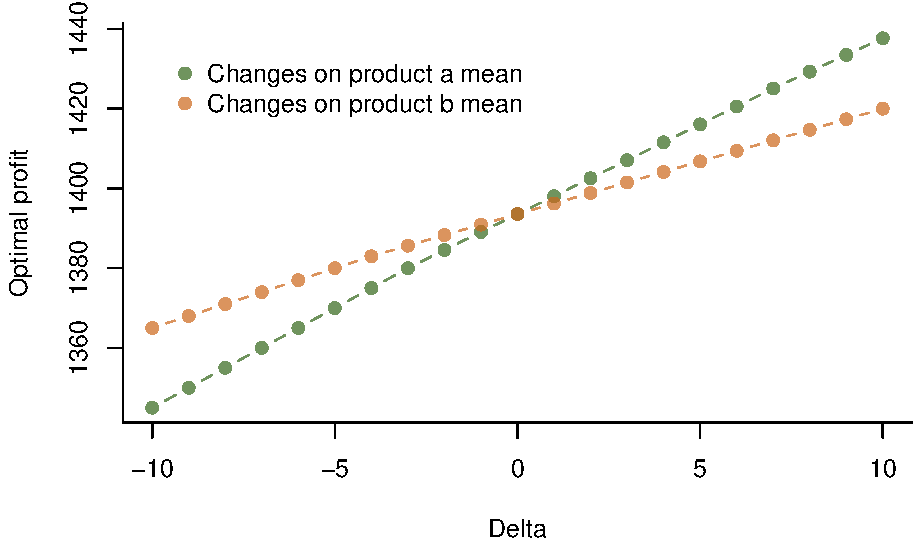
\includegraphics{Example-figure_files/figure-latex/mean-1.pdf}
\label{fig:simple1}
\end{figure}

\begin{figure}[htb]
\centering
\caption{Optimal expected profit vs.\ change in standard deviation}
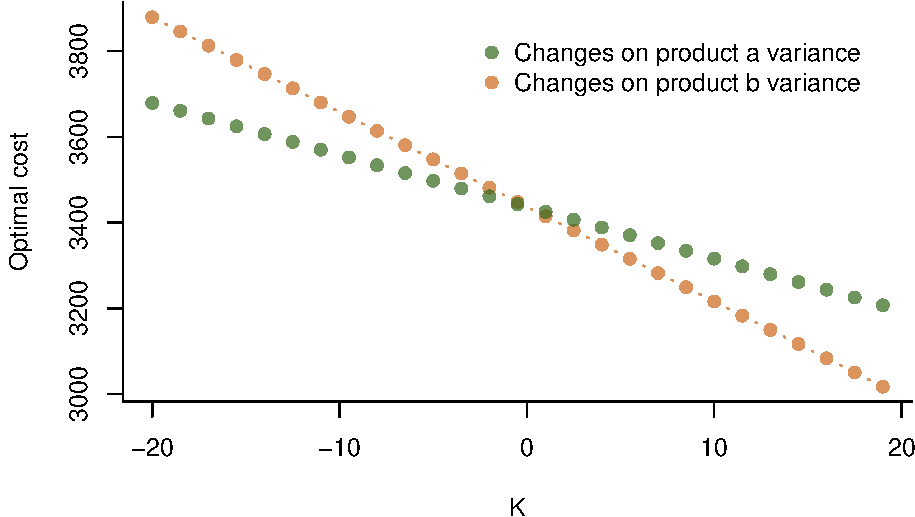
\includegraphics{Example-figure_files/figure-latex/var-1.pdf}
\label{fig:simple2}
\end{figure}

\section{Price-Setting}
\label{se:price}

We now move on the (more complex) case in which one is free to vary the prices of individual products (see \cite{De20}). Subsections \ref{sub:price1} and \ref{sub:price2} are concerned with additive and multiplicative price-demand models, respectively.

\subsection{Additive price-demand model} \label{sub:price1}

We first consider the case in which an \emph{additive} price-demand model has been used. That is, the mean demand of product $j$ can be written in the form:
\[
\mu_j = \alpha_j + \sum_{k=1}^n M_{jk} p_k.
\]

Suppose we wish to explore the effect of increasing the price of product $k$ by $\Delta$. The effect on the LP is as follows:
\begin{itemize}
\item The objective coefficient of $x_k$ increases by $\Delta$.
\item For all $j$ and $s$, the right-hand side of (\ref{eq:over}) decreases by $M_{jk} \Delta$, and the right-hand side of (\ref{eq:under}) increases by the same amount.
\end{itemize}
From this it follows that the margin is:
\[
\Delta \, x^*_k \, + \,
\Delta \sum_{j=1}^n M_{jk} \, \sum_{s \in S} \big( \pi_{sj}^u - \pi_{sj}^o \big).
\]

Unfortunately, we can no longer apply parametric programming, since we are changing objective function and constraint coefficients simultaneously. (Of course, one can simply solve the LP for several different values of $\Delta$.)

\subsection{Multiplicative price-demand model} \label{sub:price2}

Finally, we consider the case in which a \emph{multiplicative} price-demand model has been used. That is, for a given product $j$ we have:
\[
\mu_j = \alpha_j \, \Pi_{i=1}^n p_j^{\beta_{ij}},
\]
or, equivalently,
\[
\log \mu_j = \log \alpha_j \, + \sum_{j=1}^n \beta_{ij} \log p_j.
\]
Here, the $\beta_{ij}$ are the well-known
\emph{cross-price elasticities of demand} (see, e.g., \cite{FC13}).

To handle this within our framework, one can use a first-order approximation to the demand functions...


can encode the product prices in the vector $\mathbf{w}$, and encode the estimated elasticities in the parameter matrix $\mathbf{M}$. We illustrate this on an example, based on the previous one with $p_a = 8$, $p_b = 6$ and $\mu_a = \mu_b = 210$. Suppose that our elasticity matrix is:
\[
\mathbf{E} = 
\begin{pmatrix} E_{aa} & E_{ab}\\ E_{ba} & E_{bb} \end{pmatrix}
=
\begin{pmatrix} -0.6 & 0.2\\ 0.4 & -0.3 \end{pmatrix}.
\]
We would then set:
\[
\mathbf{w} = 
\begin{pmatrix} 1\\ p_a\\ p_b \end{pmatrix} =
\begin{pmatrix} 1\\ 8\\ 6 \end{pmatrix}
\]
and
\[
\begin{aligned}
&\mathbf{M} = 
\begin{pmatrix}
\alpha_a&\frac{E_{aa}}{p_a}\mu_a&\frac{E_{ab}}{p_b}\mu_a\\
\alpha_b&\frac{E_{ba}}{p_a}\mu_b&\frac{E_{bb}}{p_b}\mu_b
\end{pmatrix} =
\begin{pmatrix}
294&-15.75&7\\
189&10.5&-10.5
\end{pmatrix},
\end{aligned}
\]
where the intercepts $\alpha_a$, $\alpha_b$ can be calculated by $\mbox{\boldmath$\mu$} = \mathbf{M}\mathbf{w}$.

We also set:
\[
\mathbf{N}=
\begin{pmatrix} \sigma_{a} & 0\\
0 & \sigma_{b} \end{pmatrix}=
\begin{pmatrix} 
25 & 0\\ 
0 & 35
\end{pmatrix}
\]

We first consider the effect of price change on the expected profit. Suppose that the selling price of product $a$ was increased by $\Delta p_a$. This change would affect the objective in the LP as well as the constraints (\ref{eq:over}) and (\ref{eq:under}). Recalling that the margin will be $\mbox{\boldmath$\delta$}^T \mathbf{x}^* + \mbox{\boldmath$\gamma$}^T \mbox{\boldmath$\pi$}^*$, as long as the components of $\mbox{\boldmath$\delta$}$ and $\mbox{\boldmath$\gamma$}$ are ``sufficiently small”, we have: 
\[
\begin{aligned}
\Delta \, P_a & =
\Big( x_a^* - |S|^{-1} \sum_{s \in S} y_a^s \Big) \Delta p_a +
\sum_{j = a,b} \Delta \mu_j \, \sum_{s \in S}
\big( \pi_{sj}^u - \pi_{sj}^o \big)\\
& = \Big( x_a^* - |S|^{-1} \sum_{s \in S} y_a^s \Big) \Delta p_a +
\frac{\Delta p_a}{p_a} \sum_{j = a,b} E_{ja} \, \mu_j \, \sum_{s \in S} \big( \pi_{sj}^u - \pi_{sj}^o \big)\\
    &= 156.25 \, \Delta p_a.
\end{aligned}
\]
Applying the same method to product $b$, we obtain:
\[
\Delta \, P_b = 199.61 \, \Delta p_b.
\]
We conclude that slightly increasing the price on either product would be profitable for the retailer, and that the expected profit is more sensitive to the changes in price of product $b$ than to the changes in price of product $a$.

As in the previous subsection, we cannot use parametric programming.  Moreover, the ``ranges of validity" from the LP software are no longer reliable, de to the fact that we have used a first-order approximation of the demand curves...

computed the range of validity for our calculated values, by solving a sequence of LPs. The results are shown in Figure \ref{fig:cross}. It is apparent that the range of validity is very large for product b, and large enough to be useful for product a.

\begin{figure}[htb]
\centering
\caption{Optimal profit vs. Change of selling price}
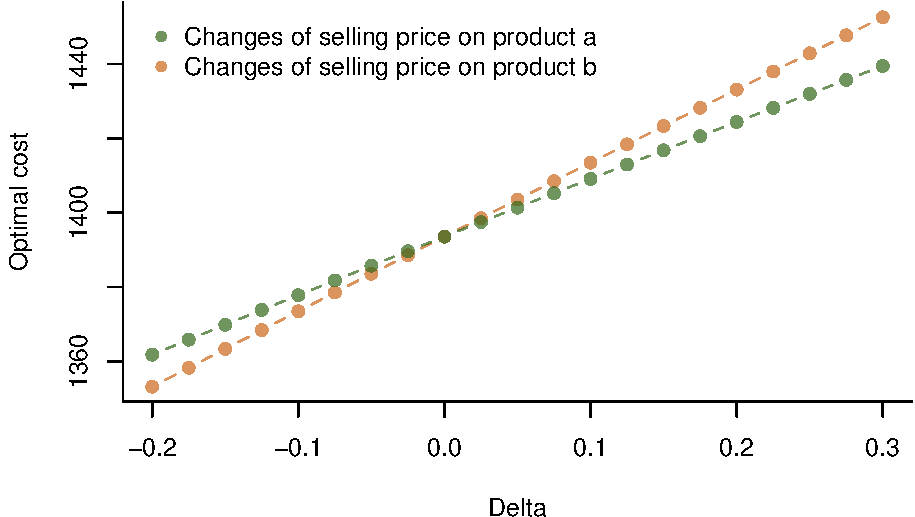
\includegraphics{Example-figure_files/figure-latex/demandunder-1.pdf}
\label{fig:cross}
\end{figure}

\subsection{Example using real-life data}
\label{sub:price3}

We now apply the approach in this section to some real-life data. Our demand data comes from a medium-sized grocery store which sells a wide range of products, many of which are perishable. The store is located in an area where customers are very sensitive to price. Therefore, the retailer wondered whether a better coordination of price-setting across products could increase the total expected profit.

The retailer was able to estimate the costs for any given product, along with the mean and standard deviation of demand. We have collected data for a sample of products. In particular, we selected the most popular product from each of the 15 most common categories (wine, eggs, tea, coffee, and so on). We assume for this specific task that demand on these products is independent. The data, selling prices and costs for these products are provided in Table \ref{tab:real_par}. Note that vegetables and meats are the most profitable products in the store, as one might expect.

\begin{table}[htb]
\centering
\caption{Data for a subset of the products}
\label{tab:real_par}
\begin{tabular}{lcc cccc}
\toprule
& \multicolumn{2}{c}{demands} & \multicolumn{4}{c}{price and costs}\\
\cmidrule(lr){2-3} \cmidrule(lr){4-7}
product & $\mu$ & $\sigma$ & $p$ & $c^1$ & $c^2$ & $c^3$\\
\midrule
beer & 119.0 & 87.5 & 2.96 & 1.78 & 0.49 & 0.51\\
wine & 32.5 & 25.7 & 11.98 & 7.13 & 2.49 & 1.33\\
tea & 27.6 & 16.8 & 5.95 & 3.65 & 0.20 & 0.36\\
bread & 87.1 & 49.8 & 0.93 & 0.63 & 0.21 & 0.05\\
eggs & 57.6 & 22.8 & 4.29 & 3.24 & 1.03 & 0.21\\
\addlinespace
fish & 44.2 & 14.1 & 2.79 & 1.75 & 1.20 & 0.49\\
fruit & 124.1 & 42.9 & 4.69 & 3.35 & 0.81 & 0.42\\
juice & 45.3 & 13.7 & 3.99 & 2.56 & 0.33 & 0.45\\
vegetables & 1197.5 & 355.09 & 2.86 & 1.96 & 0.78 & 0.56\\
tobacco & 32.8 & 24.3 & 12.99 & 9.93 & 0.31 & 0.81\\
\addlinespace
meat & 126.8 & 10.2 & 20.99 & 16.67 & 3.89 & 2.10\\
milk & 60.2 & 11.2 & 1.94 & 1.28 & 0.60 & 0.35\\
coffee & 19.5 & 9.8 & 4.93 & 3.17 & 0.44 & 0.50\\
dairy & 15.8 & 9.7 & 2.28 & 1.63 & 0.55 & 0.13\\
oil & 25.0 & 8.7 & 2.42 & 1.74 & 0.72 & 0.08\\
\bottomrule
\end{tabular}
\end{table}

There also existed 7 linear constraints. For instance, there was an upper limit on the total amount of liquid products that the retailer could store, and there were lower limits on the sizes of orders from particular brands. The detailed constraints are summarised in Appendix \ref{se:con}.

The retailer did not have information about elasticities, so we will use price elasticities and cross-price elasticities for grocery items from literature (e.g., \cite{LC03,ZW03,VD99,HPQ99}). Details on the elasticities for our selected products are given in Appendix \ref{se:ela}.

To fit this problem within our framework, we assume that
\[
\begin{aligned}
&\mathbf{M} = 
\begin{pmatrix}
\alpha_1&\frac{E_{1,1}}{p_1}\mu_1&\cdots&\frac{E_{1,n}}{p_n}\mu_1\\
\vdots&\vdots&\ddots&\vdots\\
\alpha_n&\frac{E_{n,1}}{p_1}\mu_n&\cdots&\frac{E_{n,n}}{p_n}\mu_n
\end{pmatrix}, \quad
\mathbf{w} = 
\begin{pmatrix}
1\\
p_1\\
\vdots\\
p_n
\end{pmatrix}, \\
&\mathbf{N} = 
\begin{pmatrix}
\sigma_1^e&\cdots&0\\
\vdots&\ddots&\vdots\\
0&\cdots&\sigma_n^e\\
\end{pmatrix}
\; \mbox{ and } \; 
\mbox{\boldmath$\tilde{\epsilon}$} = 
\begin{pmatrix}
\tilde{\epsilon}_1\\
\vdots\\
\tilde{\epsilon}_n
\end{pmatrix}.
\end{aligned}
\]
Here, $E_{ji}$ denotes cross elasticity of product $j$ on product $i$.

To convert the SLP into an LP, we simulated $200$ scenarios, assuming that the error terms $\tilde{\epsilon}_j$ follow independent standard normal distribution. The resulting LP had 15 $x$ variables, 3000 $y$ variables, 3000 $z$ variables, and 6007 constraints. Fortunately, such a big LP problem can be solved easily and quickly using any of several readily available solvers (e.g. 'lpSolve' package in R).

The optimal first-stage solution and the total expected profit are presented in Table \ref{tab:real_output}. We remark that, for some items, the optimal stock level is below the mean demand (compare Tables \ref{tab:real_par} and \ref{tab:real_output}). This is probably because, for those items, the over-stocking cost is higher than the under-stocking cost. One could obtain a higher service level for those items by adding constraints to the LP and re-solving. This could of course lead to a drop in the total expected profit.

\begin{table}[htb]
\centering
\caption{Optimal first-stage solution and expected profit}
\label{tab:real_output}
\resizebox{0.45\linewidth}{!}{
\begin{tabular}{cccc}
\toprule
$x_1^*$ & $x_2^*$ & $x_3^*$ & $x_4^*$\\
96.53 & 26.47 & 22.87 & 57.85\\
\hline
$x_5^*$ & $x_6^*$ & $x_7^*$ & $x_8^*$\\
40.48 & 37.45 & 101.76 & 42.21\\
\hline
$x_9^*$ & $x_{10}^*$ & $x_{11}^*$ & $x_{12}^*$\\
1036.14 & 15.06 & 120.46 & 54.78\\
\hline
$x_{13}^*$ & $x_{14}^*$ & $x_{15}^*$ & $P^*$\\
15.91 & 9.04 & 19.16 & 1224.17\\
\bottomrule
\end{tabular}}
\end{table}

Next, we explore the sensitivity of the optimal expected profit with respect to percentage changes in (a) the prices of individual products and (b) the standard deviations of the demands for individual products. The results of margins and ranges of validity for these margins, rounded to the nearest percentage point, are shown in Table \ref{tab:real_sum}.

\begin{table}[htb]
\centering
\caption{Margins of profit and Bounds for ranges of validity in \%}
\label{tab:real_sum}
\resizebox{\linewidth}{!}{
\begin{tabular}{lcc ccc}
\toprule
& \multicolumn{2}{c}{Margins of profit} & \multicolumn{3}{c}{Bounds of ranges of validity}\\
\cmidrule(lr){2-3} \cmidrule(lr){4-6}
& \% of $p_j$ increase 
& \% of $\sigma_j$ decrease
& \% of $p_j$ decrease
& \% of $p_j$ increase
& \% of $\sigma_j$ decrease\\
\midrule
beer & -0.38 & 1.25 & 1 & 1 & 7\\
wine & 2.27 & 1.15 & 3 & 2 & 14\\
tea & 1.58 & 0.45 & 10 & 15 & 100\\
bread & 0.02 & 0.24 & 5 & 6 & 100\\
egg & 0.50 & 0.39 & 19 & 14 & 100\\
fish & 0.57 & 0.24 & 6 & 5 & 100\\
fruit & 3.59 & 0.93 & 7 & 9 & 7\\
juice & 0.41 & 0.29 & 3 & 3 & 100\\
vegetable & 23.85 & 5.09 & 11 & 9 & 6\\
tobacco & 0.17 & 1.22 & 2 & 2 & 100\\
meat & 20.35 & 0.96 & 10 & 5 & 100\\
milk & 3.95 & 0.12 & 4 & 3 & 100\\
coffee & -0.18 & 0.19 & 6 & 5 & 100\\
dairy & -2.50 & 0.09 & 10 & 3 & 100\\
oil & 0.25 & 0.09 & 6 & 5 & 100
\\
\bottomrule
\end{tabular}}
\end{table}

Using the output of our procedure, we were able to provide some insights and suggestions for the retailer:
\begin{itemize}
\item Increasing the price of vegetables and/or meat is likely to yield a significant increase in the total expected profit. However, to be safe, the increases should not exceed 5\%.
\item Making other price changes may also increase the expected profit, but only slightly.
\item Improving the forecasting technique could also improve the expected profit. If the forecasting budget is limited, the retailer should first consider improving the forecasts of demand for tobacco.
\end{itemize}

%%%%%%%%%%%%%%%%%%%%
\section{Summary and Conclusion}
\label{se:conclusion}

This paper provides a new tool for coordinating marketing and inventory decisions in a retail environment. It enables one to estimate the change in expected profit that would arise from specific marketing actions, and thereby decide if those actions are worthwhile. An attractive feature of our method is that the only software tool needed is a standard linear programming solver.

Our method can be applied to any problem that can be modelled as a stochastic linear program, and therefore it could perhaps be used in contexts other than retail (e.g., manufacturing). It seems especially useful, however, for multi-product newsvendor problems that are too complex to be solved analytically. This includes, for example, problems with many linear constraints and/or correlated demands.

Our work can also be viewed as a contribution to the rapidly growing literature on Sales and Operations Planning.

%%%%%%%%%%%%%%%%%%%%%%%%%%%%%%
\printbibliography
%%%%%%%%%%%%%%%%%%%%%%%%%%%%%%
\newpage
\begin{center}
{\bf\Large Appendices}
\end{center}

\appendix

\section{Detailed Output for First Example} \label{se:report}

\begingroup\fontsize{7}{9}\selectfont
\begin{longtable}{cccccc}
\caption{Variable values, reduced costs and objective function ranges}\\
\toprule
variable & final value & reduced cost & coefficient & allowable increase & allowable decrease\\
\midrule
\endfirsthead
\multicolumn{6}{@{}l}{\textit{(continued)}}\\
\toprule
variable & final value & reduced cost & coefficient & allowable increase & allowable decrease\\
\midrule
\endhead
\
\endfoot
\bottomrule
\endlastfoot
$y_a^{1}$ & 7.14 & 0.000 & -0.833 & 0.317 & 0.5\\
$y_a^{2}$ & 0.00 & -0.833 & -0.833 & 0.833 & 10000.0\\
$y_a^{3}$ & 27.14 & 0.000 & -0.833 & 0.317 & 0.5\\
$y_a^{4}$ & 17.14 & 0.000 & -0.833 & 0.317 & 0.5\\
$y_a^{5}$ & 17.14 & 0.000 & -0.833 & 0.317 & 0.5\\
\addlinespace
$y_a^{6}$ & 0.00 & -0.833 & -0.833 & 0.833 & 10000.0\\
$y_a^{7}$ & 0.00 & -0.833 & -0.833 & 0.833 & 10000.0\\
$y_a^{8}$ & 0.00 & -0.833 & -0.833 & 0.833 & 10000.0\\
$y_a^{9}$ & 7.14 & 0.000 & -0.833 & 0.317 & 0.5\\
$y_a^{10}$ & 17.14 & 0.000 & -0.833 & 0.317 & 0.5\\
\addlinespace
$y_a^{11}$ & 0.00 & -0.833 & -0.833 & 0.833 & 10000.0\\
$y_a^{12}$ & 0.00 & -0.833 & -0.833 & 0.833 & 10000.0\\
$y_b^{1}$ & 0.00 & -0.833 & -0.833 & 0.833 & 10000.0\\
$y_b^{2}$ & 0.00 & -0.833 & -0.833 & 0.833 & 10000.0\\
$y_b^{3}$ & 10.00 & 0.000 & -0.833 & 0.607 & 0.226\\
\addlinespace
$y_b^{4}$ & 30.00 & 0.000 & -0.833 & 0.607 & 0.226\\
$y_b^{5}$ & 0.00 & -0.607 & -0.833 & 0.607 & 10000.0\\
$y_b^{6}$ & 0.00 & -0.833 & -0.833 & 0.833 & 10000.0\\
$y_b^{7}$ & 40.00 & 0.000 & -0.833 & 0.607 & 0.226\\
$y_b^{8}$ & 60.00 & 0.000 & -0.833 & 0.607 & 0.226\\
\addlinespace
$y_b^{9}$ & 30.00 & 0.000 & -0.833 & 0.607 & 0.226\\
$y_b^{10}$ & 0.00 & -0.833 & -0.833 & 0.833 & 10000.0\\
$y_b^{11}$ & 0.00 & -0.833 & -0.833 & 0.833 & 10000.0\\
$y_b^{12}$ & 0.00 & -0.833 & -0.833 & 0.833 & 10000.0\\
$z_a^{1}$ & 0.00 & -0.083 & -0.083 & 0.083 & 10000.0\\
\addlinespace
$z_a^{2}$ & 12.86 & 0.000 & -0.083 & 0.083 & 0.317\\
$z_a^{3}$ & 0.00 & -0.083 & -0.083 & 0.083 & 10000.0\\
$z_a^{4}$ & 0.00 & -0.083 & -0.083 & 0.083 & 10000.0\\
$z_a^{5}$ & 0.00 & -0.083 & -0.083 & 0.083 & 10000.0\\
$z_a^{6}$ & 2.86 & 0.000 & -0.083 & 0.083 & 0.317\\
\addlinespace
$z_a^{7}$ & 32.86 & 0.000 & -0.083 & 0.083 & 0.317\\
$z_a^{8}$ & 42.86 & 0.000 & -0.083 & 0.083 & 0.317\\
$z_a^{9}$ & 0.00 & -0.083 & -0.083 & 0.083 & 10000.0\\
$z_a^{10}$ & 0.00 & -0.083 & -0.083 & 0.083 & 10000.0\\
$z_a^{11}$ & 2.86 & 0.000 & -0.083 & 0.083 & 0.317\\
\addlinespace
$z_a^{12}$ & 32.86 & 0.000 & -0.083 & 0.083 & 0.317\\
$z_b^{1}$ & 40.00 & 0.000 & -0.250 & 0.226 & 0.607\\
$z_b^{2}$ & 20.00 & 0.000 & -0.250 & 0.226 & 0.607\\
$z_b^{3}$ & 0.00 & -0.250 & -0.250 & 0.250 & 10000.0\\
$z_b^{4}$ & 0.00 & -0.250 & -0.250 & 0.250 & 10000.0\\
\addlinespace
$z_b^{5}$ & 0.00 & 0.000 & -0.250 & 0.226 & 0.607\\
$z_b^{6}$ & 0.00 & 0.000 & -0.250 & 0.226 & 0.607\\
$z_b^{7}$ & 0.00 & -0.250 & -0.250 & 0.250 & 10000.0\\
$z_b^{8}$ & 0.00 & -0.250 & -0.250 & 0.250 & 10000.0\\
$z_b^{9}$ & 0.00 & -0.250 & -0.250 & 0.250 & 10000.0\\
\addlinespace
$z_b^{10}$ & 10.00 & 0.000 & -0.250 & 0.226 & 0.607\\
$z_b^{11}$ & 50.00 & 0.000 & -0.250 & 0.226 & 0.607\\
$z_b^{12}$ & 50.00 & 0.000 & -0.250 & 0.226 & 0.607\\
$x_a$ & 207.14 & 0.000 & 5.000 & 0.317 & 0.500\\
$x_b$ & 210.00 & 0.000 & 3.000 & 0.607 & 0.226\\*
\end{longtable}
\endgroup{}

\begingroup\fontsize{6}{9}\selectfont
\begin{longtable}{cccccc}
\caption{Shadow prices and right-hand side ranges} \\
\toprule
row & final value & shadow price & constraint RHS & allowable increase & allowable decrease\\
\midrule
\endfirsthead
\multicolumn{6}{@{}l}{\textit{(continued)}}\\
\toprule
row & final value & shadow price & constraint RHS & allowable increase & allowable decrease\\
\midrule
\endhead
\
\endfoot
\bottomrule
\endlastfoot
time\_A & 2088.6 & 0.0 & 2200 & 10000.0 & 111.4\\
time\_B & 2500.0 & 0.071 & 2500 & 20.0 & 50.0\\
time\_C & 3337.1 & 0.0 & 3500 & 10000.0 & 162.9\\
over\_a\textasciicircum{}1 & 200.0 & 0.833 & 200 & 7.1 & 10000.0\\
over\_a\textasciicircum{}2 & 207.1 & 0.0 & 220 & 10000.0 & 12.9\\
\addlinespace
over\_a\textasciicircum{}3 & 180.0 & 0.833 & 180 & 27.1 & 10000.0\\
over\_a\textasciicircum{}4 & 190.0 & 0.833 & 190 & 17.1 & 10000.0\\
over\_a\textasciicircum{}5 & 190.0 & 0.833 & 190 & 17.1 & 10000.0\\
over\_a\textasciicircum{}6 & 207.1 & 0.0 & 210 & 10000.0 & 2.9\\
over\_a\textasciicircum{}7 & 207.1 & 0.0 & 240 & 10000.0 & 32.9\\
\addlinespace
over\_a\textasciicircum{}8 & 207.1 & 0.0 & 250 & 10000.0 & 42.9\\
over\_a\textasciicircum{}9 & 200.0 & 0.833 & 200 & 7.1 & 10000.0\\
over\_a\textasciicircum{}10 & 190.0 & 0.833 & 190 & 17.1 & 10000.0\\
over\_a\textasciicircum{}11 & 207.1 & 0.0 & 210 & 10000.0 & 2.9\\
over\_a\textasciicircum{}12 & 207.1 & 0.0 & 240 & 10000.0 & 32.9\\
\addlinespace
under\_a\textasciicircum{}1 & 207.1 & 0.0 & 200 & 7.1 & 10000.0\\
under\_a\textasciicircum{}2 & 220.0 & 0.083 & 220 & 10000.0 & 12.9\\
under\_a\textasciicircum{}3 & 207.1 & 0.0 & 180 & 27.1 & 10000.0\\
under\_a\textasciicircum{}4 & 207.1 & 0.0 & 190 & 17.1 & 10000.0\\
under\_a\textasciicircum{}5 & 207.1 & 0.0 & 190 & 17.1 & 10000.0\\
\addlinespace
under\_a\textasciicircum{}6 & 210.0 & 0.083 & 210 & 10000.0 & 2.9\\
under\_a\textasciicircum{}7 & 240.0 & 0.083 & 240 & 10000.0 & 32.9\\
under\_a\textasciicircum{}8 & 250.0 & 0.083 & 250 & 10000.0 & 42.9\\
under\_a\textasciicircum{}9 & 207.1 & 0.0 & 200 & 7.1 & 10000.0\\
under\_a\textasciicircum{}10 & 207.1 & 0.0 & 190 & 17.1 & 10000.0\\
\addlinespace
under\_a\textasciicircum{}11 & 210.0 & 0.083 & 210 & 10000.0 & 2.9\\
under\_a\textasciicircum{}12 & 240.0 & 0.083 & 240 & 10000.0 & 32.9\\
over\_b\textasciicircum{}1 & 210.0 & 0.0 & 250 & 10000.0 & 40.0\\
over\_b\textasciicircum{}2 & 210.0 & 0.0 & 230 & 10000.0 & 20.0\\
over\_b\textasciicircum{}3 & 200.0 & 0.833 & 200 & 10.0 & 10000.0\\
\addlinespace
over\_b\textasciicircum{}4 & 180.0 & 0.833 & 180 & 30.0 & 10000.0\\
over\_b\textasciicircum{}5 & 210.0 & 0.226 & 210 & 0.0 & 4.0\\
over\_b\textasciicircum{}6 & 210.0 & 0.0 & 210 & 10000.0 & 0.0\\
over\_b\textasciicircum{}7 & 170.0 & 0.833 & 170 & 40.0 & 10000.0\\
over\_b\textasciicircum{}8 & 150.0 & 0.833 & 150 & 60.0 & 10000.0\\
\addlinespace
over\_b\textasciicircum{}9 & 180.0 & 0.833 & 180 & 30.0 & 10000.0\\
over\_b\textasciicircum{}10 & 210.0 & 0.0 & 220 & 10000.0 & 10.0\\
over\_b\textasciicircum{}11 & 210.0 & 0.0 & 260 & 10000.0 & 50.0\\
over\_b\textasciicircum{}12 & 210.0 & 0.0 & 260 & 10000.0 & 50.0\\
under\_b\textasciicircum{}1 & 250.0 & 0.25 & 250 & 10000.0 & 40.0\\
\addlinespace
under\_b\textasciicircum{}2 & 230.0 & 0.25 & 230 & 10000.0 & 20.0\\
under\_b\textasciicircum{}3 & 210.0 & 0.0 & 200 & 10.0 & 10000.0\\
under\_b\textasciicircum{}4 & 210.0 & 0.0 & 180 & 30.0 & 10000.0\\
under\_b\textasciicircum{}5 & 210.0 & 0.25 & 210 & 10000.0 & 0.0\\
under\_b\textasciicircum{}6 & 210.0 & 0.25 & 210 & 10000.0 & 0.0\\
\addlinespace
under\_b\textasciicircum{}7 & 210.0 & 0.0 & 170 & 40.0 & 10000.0\\
under\_b\textasciicircum{}8 & 210.0 & 0.0 & 150 & 60.0 & 10000.0\\
under\_b\textasciicircum{}9 & 210.0 & 0.0 & 180 & 30.0 & 10000.0\\
under\_b\textasciicircum{}10 & 220.0 & 0.25 & 220 & 10000.0 & 10.0\\
under\_b\textasciicircum{}11 & 260.0 & 0.25 & 260 & 10000.0 & 50.0\\
\addlinespace
under\_b\textasciicircum{}12 & 260.0 & 0.25 & 260 & 10000.0 & 50.0\\*
\end{longtable}
\endgroup{}

\section{Constraints for Real-Life Example} \label{se:con}

\begin{table}[H]
\centering
\caption{Constraints for real-life case}
\resizebox{\linewidth}{!}{
\begin{tabular}{ccccccccccccccccc}
\toprule
beer & wine & tea & bread & egg & fish & fruit & juice & vegetable & tobacco & meat & milk & coffee & dairy & oil & direction & RHS\\
\midrule
1 & 1 & 0 & 0 & 0 & 0 & 0 & 0 & 0 & 0 & 0 & 0 & 0 & 0 & 0 & $<=$ & 120\\
0 & 0 & 0 & 0 & 0 & 0 & 1 & 0 & 1 & 0 & 0 & 0 & 0 & 0 & 0 & $<=$ & 1200\\
0 & 0 & 0 & 1 & 0 & 1 & 1 & 0 & 0.1 & 0 & 1 & 1 & 0 & 1 & 0 & $<=$ & 550\\
0 & 0 & 1 & 0 & 0 & 0 & 0 & 0 & 0 & 0 & 0 & 0 & 1 & 0 & 0 & $>=$ & 30\\
0 & 0 & 0 & 0 & 0 & 0 & 0 & 0 & 0 & 0 & 0 & 0 & 0 & 0 & 1 & $<=$ & 30\\
1 & 1 & 0 & 0 & 0 & 0 & 0 & 1 & 0 & 0 & 0 & 1 & 0 & 0 & 1 & $<=$ & 300\\
0 & 0 & 0 & 0 & 1 & 0 & 0 & 0 & 0 & 0 & 0 & 0 & 0 & 0 & 0 & $<=$ & 60\\
\bottomrule
\end{tabular}}
\end{table}

\section{Elasticities for Real-Life Example} \label{se:ela}

\begin{table}[H]
\centering
\caption{Cross-price elasticities for 15 key products}
\resizebox{\linewidth}{!}{
\begin{tabular}{lccccccccccccccc}
\toprule
\multicolumn{1}{c}{\textbf{}} & \multicolumn{15}{c}{\textbf{price}} \\
\cmidrule(l{3pt}r{3pt}){2-16}
  & beer & wine & tea & bread & egg & fish & fruit & juice & vegetable & tobacco & meat & milk & coffee & dairy & oil\\
\midrule
beer & -1.98 & 0.74 & 0.33 & 0.00 & 0.00 & 0.00 & 0.00 & 0.00 & 0.00 & -0.02 & 0.19 & 0.00 & 0.00 & 0.00 & 0.00\\
wine & -0.21 & -0.84 & 0.12 & 0.00 & 0.00 & 0.00 & 0.00 & 0.00 & 0.00 & -0.02 & 0.19 & 0.00 & 0.00 & 0.00 & 0.00\\
tea & 0.10 & -0.08 & 0.03 & 0.00 & 0.00 & 0.00 & 0.00 & 0.00 & 0.00 & 0.00 & 0.00 & 0.03 & 0.00 & 0.00 & 0.00\\
bread & 0.00 & 0.00 & 0.00 & 0.06 & -0.03 & -0.05 & -0.01 & 0.00 & -0.05 & 0.00 & 0.00 & 0.00 & 0.00 & -0.01 & 0.00\\
egg & 0.00 & 0.00 & 0.00 & -0.23 & -0.22 & -0.04 & -0.06 & 0.07 & -0.03 & 0.00 & 0.04 & -0.09 & 0.01 & -0.08 & 0.01\\
\addlinespace
fish & 0.00 & 0.00 & 0.00 & -0.15 & -0.05 & -0.53 & 0.00 & -0.06 & 0.01 & 0.00 & 0.02 & -0.16 & -0.02 & -0.04 & -0.01\\
fruit & 0.00 & 0.00 & 0.00 & -0.09 & -0.04 & 0.00 & -0.60 & -0.04 & -0.03 & 0.00 & 0.00 & 0.30 & 0.04 & -0.08 & 0.04\\
juice & 0.00 & 0.00 & -0.03 & -0.06 & 0.00 & -0.09 & -0.06 & -0.85 & 0.00 & 0.00 & 0.00 & 0.14 & -0.02 & -0.05 & 0.00\\
vegetable & 0.00 & 0.00 & 0.00 & 0.00 & 0.00 & 0.00 & 0.10 & 0.00 & -0.54 & -0.04 & 0.01 & 0.20 & 0.01 & -0.03 & 0.02\\
tobacco & -0.07 & -0.07 & 0.00 & 0.00 & 0.00 & 0.00 & 0.00 & 0.00 & 0.03 & 0.07 & 0.05 & 0.00 & 0.00 & 0.00 & 0.00\\
\addlinespace
meat & 0.01 & 0.01 & 0.00 & 0.00 & 0.02 & 0.08 & -0.04 & 0.00 & -0.02 & 0.04 & -0.48 & 0.17 & 0.00 & -0.23 & 0.05\\
milk & 0.00 & 0.00 & 0.01 & 0.00 & -0.12 & -0.01 & 0.07 & 0.08 & 0.08 & 0.00 & 0.02 & -0.96 & 0.01 & 0.00 & -0.01\\
coffee & 0.00 & 0.00 & 0.00 & 0.00 & 0.01 & 0.00 & 0.03 & 0.00 & -0.04 & 0.00 & 0.00 & 0.03 & 0.60 & 0.00 & 0.00\\
dairy & 0.00 & 0.00 & 0.00 & -0.04 & -0.01 & -0.01 & -0.01 & 0.00 & -0.01 & 0.00 & -0.07 & 0.00 & 0.00 & -0.55 & 0.00\\
oil & 0.00 & 0.00 & 0.00 & 0.00 & 0.00 & -0.02 & 0.01 & 0.00 & 0.03 & 0.00 & 0.09 & 0.04 & 0.00 & 0.00 & -0.70\\
\bottomrule
\end{tabular}}
\end{table}

\end{document}